% ---------------------------------------------------------------
% TEMPLATE TCC2 - SENAC SANTO AMARO
% ---------------------------------------------------------------
% Trabalho de Conclusão de Curso 2
% ---------------------------------------------------------------

\documentclass[
    12pt,
    openright,
    oneside,
    a4paper,
    english,
    brazil
]{abntex2}

\usepackage{lmodern}
\usepackage[T1]{fontenc}
\usepackage[utf8]{inputenc}
\usepackage{lastpage}
\usepackage{indentfirst}
\usepackage{color}
\usepackage{graphicx}
\usepackage{microtype}
\usepackage{float}
\usepackage{booktabs}
\usepackage{multirow}
\usepackage{longtable}
\usepackage{amsmath,amssymb}
\usepackage[brazilian,hyperpageref]{backref}
\usepackage[alf]{abntex2cite}
\usepackage{array}
\usepackage{tabularx}
\usepackage{pdflscape}
\usepackage{geometry}

\definecolor{blue}{RGB}{41,5,195}

\newcolumntype{Y}{>{\raggedright\arraybackslash}X}

\makeatletter
\hypersetup{
    pdftitle={\@title},
    pdfauthor={\@author},
    pdfsubject={TCC2 - SENAC Santo Amaro},
    pdfcreator={LaTeX with abnTeX2},
    pdfkeywords={tcc2}{senac}{santo amaro}{trabalho de conclusão},
    colorlinks=true,
    linkcolor=blue,
    citecolor=blue,
    filecolor=magenta,
    urlcolor=blue,
    bookmarksdepth=4
}
\makeatother

\titulo{Otimização do tempo total do processo de avaliação neuropsicológica utilizando Simulação de eventos discretos e Teoria das filas}
\autor{Caio Troiano Collino (1142491237) \\ Thiago Pereira Lins da Silva (1142515180) \\ Vinícius Vianna Egydio de Carvalho (1142446597)}
\local{São Paulo}
\data{2026}
\orientador{Prof. Alessandro Ranulfo Lima Nery}
\tipotrabalho{Trabalho de Conclusão de Curso II}
\instituicao{%
  SENAC -- Serviço Nacional de Aprendizagem Comercial
  \par
  Unidade Santo Amaro
  \par
  Curso de Bacharelado em Ciência da Computação
}
\preambulo{Trabalho de Conclusão de Curso II apresentado ao SENAC Santo Amaro como requisito para conclusão do curso de Bacharelado em Ciência da Computação.}

\makeindex

\begin{document}

\selectlanguage{brazil}
\frenchspacing

\pretextual

\imprimircapa
\imprimirfolhaderosto

\begin{resumo}
Este documento apresenta a proposta inicial do Trabalho de Conclusão de Curso (TCC1) desenvolvido no SENAC Santo Amaro. O objetivo deste trabalho é demonstrar que um modelo estatístico pode reduzir o tempo mínimo necessário para a obtenção da devolução de um diagnóstico neuropsicológico. A justificativa para este estudo baseia-se na dificuldade de acesso dos pacientes a tratamentos e adaptações necessários devido a atrasos no diagnóstico e na lacuna existente na aplicação de métodos de otimização computacional no contexto dessa avaliação. A revisão bibliográfica abrange principalmente Pesquisa operacional, Teoria das filas e Simulação de eventos discretos. Como solução proposta, pretende-se criar um modelo de processos capaz de representar as etapas essenciais do diagnóstico e simular as mesmas, utilizando como ferramenta principal Python e bibliotecas do mesmo, como Pandas, NumPy e SimPy. Este trabalho está organizado em três capítulos que apresentam a introdução ao tema, a revisão bibliográfica que fundamenta a pesquisa, o desenvolvimento com a solução proposta e o cronograma de trabalho, seguidos das referências bibliográficas.
\end{resumo}

\begin{resumo}[Abstract]
This document follows the TCC structure proposed by Wazlawick for Computer Science, emphasizing the research problem, objectives, proposed method, development details, and scientific analysis of results.
\end{resumo}

\tableofcontents*
\cleardoublepage

\textual

% ---------------------------------------------------------------
% INTRODUÇÃO
% ---------------------------------------------------------------
\chapter{Introdução}

Este trabalho tem como tema o uso de métricas e parâmetros em um modelo de simulação de modo que auxilie nas tomadas de decisões que envolvem a otimização do tempo total da entrega do diagnóstico neuropsicológico, considerando que o mesmo parte de uma suspeita inicial, passa pela busca de um profissional especializado, e finaliza com a devolução do diagnóstico. Esse processo é denominado de avaliação neuropsicológica, e consiste em uma investigação estruturada a partir de uma bateria de testes e entrevistas em múltiplas etapas extensas para confirmar ou refutar a suspeita inicial, no qual é feito em uma clinica especializada que possui um fluxo de pacientes.

\section{Contextualização do problema}

No presente momento de desenvolvimento deste trabalho, observa-se uma grande procura por avaliações neuropsicológicas: 69,6\% dos diagnósticos de autismo foram entre 2020 e 2024 \cite{Mab2026}. A principal causa para essa busca reside na maior divulgação do tema em mídias tradicionais e digitais, especialmente em discussões relacionadas ao Transtorno do Espectro Autista (TEA) e outros transtornos do neurodesenvolvimento. Na figura abaixo, podemos observar o crescimento de diagnósticos por ano:

\begin{figure}[H]
	\caption{Ano do diagnóstico}
	\centering
	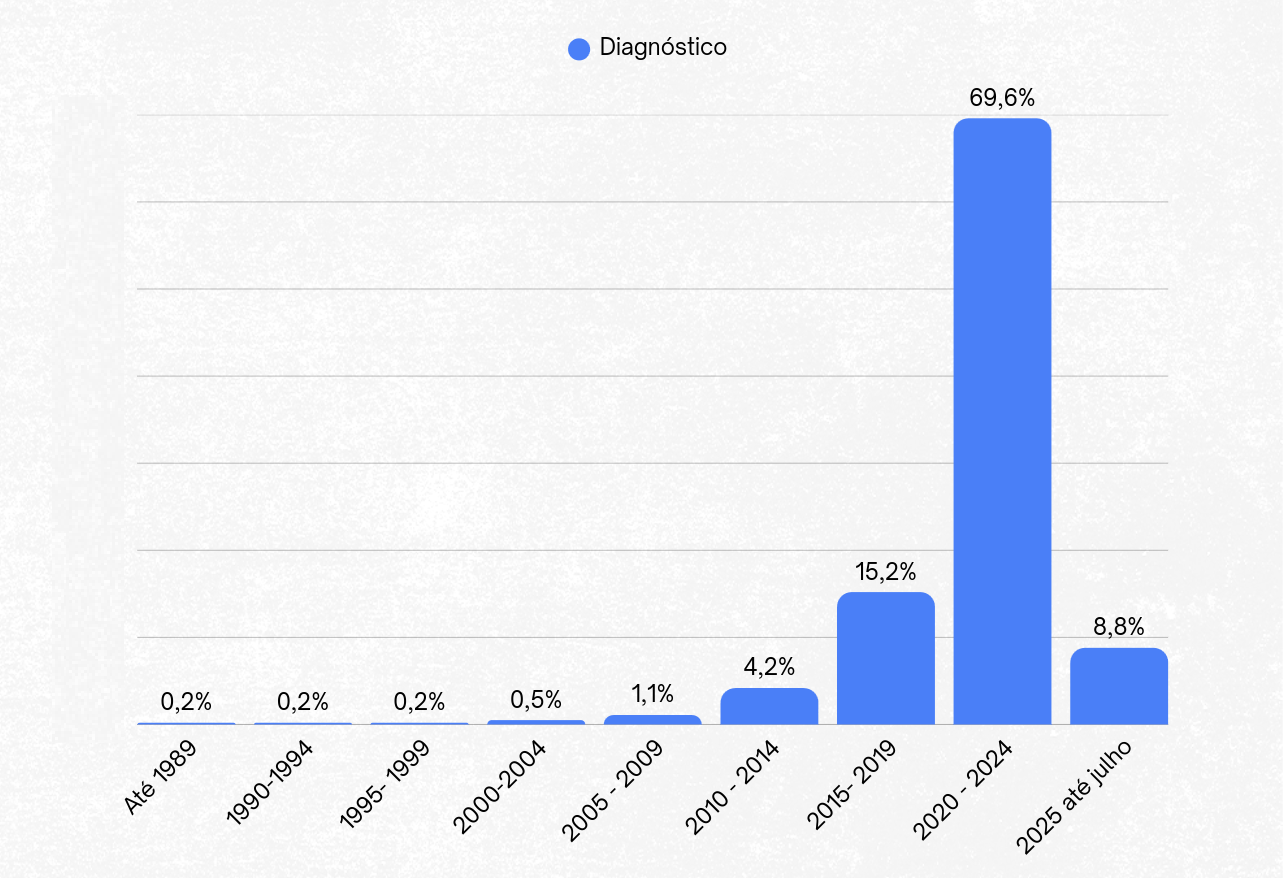
\includegraphics[width=15cm]{assets/ano_do_diagnostico_mab.png}
	\label{fig:ano_diagnostico}
	\legend{Fonte: \citeonline{Mab2026}}
\end{figure}

Contudo, quando uma pessoa busca por esse tipo de avaliação, ela constantemente se depara com longas filas de espera, um processo que excede o tempo esperado e até um intervalo maior que um ano desde a suspeita inicial até a devolução do diagnóstico. O período de espera até a conclusão do processo é um problema sério e relevante, já que pode atrasar tratativas como: intervenções, tratamentos, adaptações escolares, acadêmicas, profissionais e sociais.

Ademais, a falta de uma organização clara e processos bem definidos pode tornar o diagnóstico mais vulnerável a atrasos em múltiplas etapas. Considerando esse cenário, a computação pode ter uma contribuição significativa na análise, na modelagem e na melhoria do processo, tornando possível a identificação de gargalos a partir de insumos e métricas gerados pela simulação de cenários, que podem auxiliar na proposição de estratégias adequadas para tornar o fluxo de atendimento mais eficiente.

\section{Formulação do problema}
Coloque o problema em forma de pergunta clara, delimitando o que será investigado e qual resultado se espera atingir dentro da Computação.

\section{Objetivos e hipótese}

Separamos os objetivos entre objetivo geral, no qual é a meta a ser atingida por este trabalho. Já os objetivos específicos, são os meios no qual desenvolveremos esta pesquisa.

\subsection{Objetivo geral}
% Declare o propósito principal do TCC2 em uma frase direta, conectando-o ao problema e deixando claro se o foco é compreender, comparar, validar ou propor algo novo.

Analisar quais fatores podem impactar negativamente ou positivamente na redução do tempo total do paciente dentro do processo de avaliação neuropsicológica, considerando que o mesmo incorpora desde a primeira consulta até o retorno com o resultado do diagnóstico, através de um modelo de simulação de eventos discretos baseado em conceitos de pesquisa operacional, como por exemplo teoria das filas.

\subsection{Objetivos específicos}
% Liste objetivos mensuráveis que estruturam o plano de trabalho. Tente utilizar verbos como revisar, comparar, modelar, quantificar ou validar. Exemplos:
% \begin{itemize}
%     \item Revisar obras-chave sobre [tema] e identificar lacunas;
%     \item Modelar ou prototipar a abordagem proposta;
%     \item Implementar experimentos controlados;
%     \item Avaliar o desempenho por métricas (ex.: acurácia, latência).
% \end{itemize}


Para o atingir o objetivo geral, serão realizadas as seguintes etapas:
\begin{itemize}
		\item Mapeamento da linha de processos realizados na avaliação;
		\item Construção de um modelo de processos;
		\item Desenvolvimento de um simulador capaz de reproduzir os processos;
		\item Realização de simulações com o modelo criado, com o intuito de reproduzir diversos cenários e obter suas métricas;
		\item Análise dos resultados obtidos através das simulações, observando quais parâmetros possui maior impacto positivo ou negativo com base nas métricas retiradas.
\end{itemize}

O mapeamento auxilia a compreensão do funcionamento do processo, tornando viável o reconhecimento de pontos críticos, que podem causar atrasos e falhas capazes de comprometer o tempo de diagnóstico. Essa análise torna plausível a identificação de possíveis fatores que impactam os cenários, ou seja, quais parâmetros podem ser prováveis ofensores para o processo. Além disso, este tempo de espera pode estar presente em diversos momentos do processo, como na fila para o atendimento inicial, no intervalo entre a realização dos exames, na devolução do diagnóstico ou em outras fases intermediárias. Embora o mapeamento permita a identificação das etapas críticas, ele não é suficiente para estimar o impacto de alterações nos recursos, como o aumento de número de profissionais.

Com isso, será construído um modelo de processos capaz de representar o funcionamento do mesmo. Esse modelo deve ser capaz de testar múltiplos cenários, tornando possível a avaliação de como mudanças na distribuição de recursos ou no fluxo de pacientes podem impactar o tempo de espera dos diagnósticos. Após a criação do modelo e do desenvolvimento do simulador, serão realizadas simulações com o intuito de observar como o modelo se comporta em diferentes condições. Por último, em função dos resultados obtidos nas simulações, será analisado quais parâmetros mais impactaram de forma positiva o cenário simulado.

\subsection{Hipótese ou critério de validação}
% Descreva a hipótese que será testada ou o critério usado para afirmar que o objetivo geral foi atingido. Caso não haja hipótese formal, explique como as métricas escolhidas demonstrarão o sucesso esperado.

Através das simulações e das métricas retornadas, será identificado qual ou quais são os principais ofensores na eficiência do processo de avaliação neuropsicológica em uma clínica especializada. Espera-se que ao ajustar um ou mais parâmetros, seja possível reduzir o tempo de espera total dos pacientes, além de trazer insumos tanto sobre o cenário real quanto sobre os cenários simulados, de forma que seja possível trazer benefícios à clínica que deseja simular o seu próprio funcionamento.

\section{Justificativa}
% Ressalte a importância do problema para a Computação, destacando contribuições acadêmicas, sociais ou industriais. Explique como a proposta evita se tornar um “manual de ferramenta”.

Por mais que existam trabalhos presentes na área acadêmica relacionados ao estudo de fluxos de trabalho em processos diagnósticos \cite{Galves2022,Silva2023}, muitos deles são direcionados a locais específicos, diagnósticos específicos ou contextos clínicos restritos. Como um processo amplo capaz de auxiliar na formação de diferentes diagnósticos, a avaliação neuropsicológica ainda é pouco explorada em um contexto de otimização computacional.

Assim sendo, este trabalho se justifica a partir de sua relevância social, acadêmica e prática, além de facilitar a reprodutibilidade de cenários que utilizem o mesmo modelo, mas não se limitando à uma clínica específica. Atrasos ou ausências de diagnósticos podem resultar em impactos significativos na vida dos pacientes, especialmente em um contexto escolar, acadêmico, profissional e social. Tanto crianças quanto adultos estão vulneráveis a esses impactos, tornando difícil o acesso a intervenções adequadas, adaptações necessárias e acompanhamento terapêutico.

A realização de diagnósticos em momentos adequados possibilita o início de tratamentos, terapias, adaptações pedagógicas e outras formas de suporte para o paciente. Portanto, busca-se estudar meios capazes de reduzir o tempo total do processo de diagnóstico de forma que não afete o tempo mínimo necessário para garantir precisão, qualidade e confiabilidade na avaliação.

% ---------------------------------------------------------------
% REVISÃO BIBLIOGRÁFICA
% ---------------------------------------------------------------
\chapter{Revisão Bibliográfica / Trabalhos Relacionados}

\section{Fundamentos teóricos necessários}
% Explique os conceitos essenciais, definindo termos e equações quando necessário. Utilize blocos de texto ou pequenos quadros comparativos para sintetizar modelos.

% Um exemplo de citação direta poderia ser `\citeonline{Silva2022}` para reforçar que determinados métodos exigem validação empírica; uma citação indireta pode ser escrita como “vários estudos destacam ...” seguido de `\cite{Wazlawick2020}`.

Nesta seção, apresentaremos quais são os principais conceitos que são necessários para o desenvolvimento deste trabalho.

\subsection{Pesquisa Operacional}
A Pesquisa Operacional (PO) é uma ciência aplicada voltada para a resolução de problemas reais que objetiva fornecer ferramentas quantitativas ao processo de tomada de decisões \cite{Rodriguez2009}. Dentre as diversas técnicas existentes de PO, utilizaremos Simulação de Eventos e Teoria das filas, que serão essenciais no nosso contexto para a reprodução de cenários e a construção de modelos.

\subsection{Simulação de Eventos}

Segundo \citeonline{Lieberman2013}, Simulação é uma das técnicas com maior destaque por ser uma ferramenta flexível, poderosa e intuitiva. Essa técnica envolve a utilização de um computador para imitar a operação de um processo inteiro ou sistema, podendo ser utilizado em diversos cenários, como a análise de riscos em processos financeiros, simulando a evolução de transações envolvidas para gerar um quadro de possíveis resultados. O registro do desempenho de operações simuladas torna possível  a avaliação e a comparação de alternativas antes de escolher uma delas. Existem dois tipos de simulação: simulação de eventos discretos e simulação de eventos contínuos.

Na simulação por eventos discretos, as mudanças no estado do sistema ocorrem de maneira instantânea em pontos aleatórios no tempo como o resultado da ocorrência desses eventos discretos. Por exemplo: em um sistema de filas onde o estado do sistema é o número de clientes no sistema, os eventos discretos responsáveis por mudar esse estado são a chegada e a saída de um cliente em decorrência da finalização do serviço.

Na simulação contínua, as mudanças no estado do sistema ocorrem de maneira contínua ao longo do tempo. Por exemplo: assumindo que o sistema de interesse seja um avião em voo e seu estado seja a posição atual da aeronave, o estado irá mudar continuamente ao longo do tempo.

Utilizaremos simulação por eventos discretos, já que ela condiz melhor com o nosso tema. No contexto de uma clínica, os eventos discretos que irão mudar o estado do sistema será a chegada e saída de clientes após a conclusão da sessão.

\subsection{Teoria das Filas}

Segundo \citeonline{Lieberman2013}, a teoria das filas é o estudo da espera em formas diversas, como a compra de um ingresso para um sessão de cinema ou fazer um depósito bancário. Ter de esperar em uma fila não é limitado apenas a transtornos pessoais não tão significantes: deixar máquinas a espera para serem reparadas pode gerar perdas na produção e aviões que aguardam para decolar ou pousar podem afetar horários de voos futuros.

Modelos de filas são a principal ferramenta utilizada para a representação de sistemas de filas, com fórmulas para cada modelo responsáveis por indicar o funcionamento e o tempo médio de espera do mesmo em uma determinada série de circunstâncias. Utilizaremos modelos de fila que possuem as determinadas características: um único canal e uma única fila, um único canal e múltiplas filas, vários canais e uma única fila e vários canais e múltiplas filas. Em múltiplos cenários, utilizaremos os modelos de fila citados, com o intuito de encontrar o modelo ideal para encontrar o melhor tempo possível no processo de diagnóstico.

\subsection{Métricas}

Como métricas, temos: tempo de fila, tamanho da fila, tempo de atendimento, tempo de espera entre processos e tempo total de processo. Tempo de fila é o tempo de espera até o atendimento inicial. Tamanho da fila é o número de pessoas esperando por atendimento. Tempo de atendimento é a duração de um atendimento. Tempo de espera é a quantidade de tempo entre um atendimento e outro. Tempo total de processo é o tempo total até o diagnóstico. 

\subsection{Parâmetros}

Como parâmetros, temos: número de seções, número de profissionais e disponibilidade médica. Número de seções é o número de atendimentos necessários para realizar um diagnóstico. Número de profissionais é a quantidade de profissionais disponíveis. Disponibilidade média é o quantidade de profissionais disponíveis.

\subsection{DSM 5}
% OBS: Incompleto, polir e completar depois

O Manual diagnóstico e estatístico de transtornos mentais (DSM), segundo a \citeonline{Apa2023}, é a principal ferramenta utilizada no diagnóstico neuropsicológico, servindo como uma classificação dos transtornos mentais e critérios associados, elaborada de modo que seja facilitado o diagnóstico confiável desses transtornos.

Utilizaremos o DSM para compreender o processo diagnóstico de certos transtornos, facilitando a modelagem na simulação e durante a triagem.

\subsection{Avaliação Neuropsicológica}
% OBS: Não tenho certeza se a primeira citação deve ser em relação ao próprio livro ou o autor referenciado pelo livro

Segundo \citeonline{Malloy2018}, uma avaliação, empreendida com fins profissionais, é a descrição de aspectos relevantes de uma pessoa através de técnicas e teorias científicas particulares, com o fim de responder questões específicas. De forma generalizada, uma avaliação deve atender diferentes propósitos, como a descrição do funcionamento atual do indivíduo(ressaltando suas forças e dificuldades), de sua capacidade de viver de modo autônomo e independente e as possibilidades de adaptação social, profissional e pessoal do mesmo, levando em consideração a minimização de seu sofrimento físico e psicológico. Além disso, a avaliação deve identificar necessidades terapêuticas, recomendar intervenções e apontar resultados possíveis destas e contribuir para o diagnóstico diferencial de distúrbios emocionais, cognitivos e comportamentais. A avaliação também pode monitorar a evolução do tratamento e identificar novas questões que possam requerer atenção profissional. Por último, segundo o \citeonline{Meyer2001}, devolutivas devem ser oferecidas de maneira competente e empática a respeito dos resultados de todo o processo. 

A avaliação neuropsicológica, segundo \citeonline{Malloy2018}, é uma atividade emergente do campo da neuropsicologia, se tratando de um método capaz de investigar as funções cognitivas e o comportamento de um indivíduo, relacionando-os com o funcionamento normal ou deficitário do sistema nervoso central (SNC), de modo que seja possível o diagnóstico, determinação da natureza ou etiologia dos sintomas, a gravidade das sequelas, o prognóstico, a evolução do caso e o oferecimento de bases que contribuam para a reabilitação.

\section{Técnicas, métodos ou abordagens existentes}
Apresente abordagens já empregadas no contexto e destaque o que funcionou ou falhou. Inclua uma tabela comparativa simples para clarificar diferenças:
\begin{table}[htb]
  \centering
  \caption{Comparativo de abordagens relacionadas}
  \begin{tabular}{p{4cm}p{3cm}p{4cm}}
    \toprule
    Abordagem & Domínio & Limitação principal \\
    \midrule
    Técnica A & IoT & Falta de validação em larga escala \\
    Técnica B & Redes neurais & Alto custo computacional \\
    \bottomrule
  \end{tabular}
  \legend{Tabela ilustrativa com limitações observadas.}
\end{table}

\section{Trabalhos correlatos e limitações}
% Liste artigos diretamente relacionados e explique por que cada um não resolve totalmente o problema (ex.: falta de comparação, escopo diferente, dados limitados). Relacione essas lacunas com o que sua pesquisa pretende preencher.

% \textit{Evite a “síndrome da intersecção esquecida”: inclua trabalhos que aplicaram a técnica na mesma área.}

Com base no problema deste trabalho, e em sua proposta de solução, foram encontrados 3 artigos relevantes, com problemas e soluções semelhantes.

\subsection{Trabalho 1: Redução do tempo de espera para realização de avaliação neuropsicológica: um projeto de intervenção \cite{Silva2023}}

Este trabalho abordou o problema de tempo de espera dos pacientes. Nele, é identificado que a avaliação neuropsicológica é uma demanda que existe, mas não é devidamente atendida, resultando em excesso de atendimentos e tempos de espera de até 1 ano.

Além disso, o trabalho apresenta como proposta de solução a aplicação de práticas a serem seguidas, como a padronização de laudos, a utilização de triagem telefônica e a redução do uso da quantidade de testes.

A principal diferença entre este trabalho e o nosso, é a proposta de solução. Enquanto o trabalho 1 apresenta soluções administrativas nas quais os testes foram feitos de forma empírica e sem apresentação de dados estatísticos, o nosso trabalho propõe a construção de um modelo estatístico e com simulação de cenários.

\subsection{Trabalho 2: Estudo de caso da aplicação de simulação de eventos discretos num processo de radioterapia \cite{Galves2022}}

O trabalho 2 aplica a simulação de eventos discretos em um processo de exame de radioterapia, onde há a modelagem do processo como um todo. Nele, é feito o modelo das filas hospitalares, aplicando simulações para identificar gargalos na operação com o objetivo de detectar melhorias a serem feitas na operação.

Os autores propõem como solução o uso de simulação de eventos discretos nos softwares SIMUL8 e ARENA, a partir de amostra de dados de pacientes da clínica que foram analisados e tratados. Com isso, foi possível analisar as distribuições e as expressões que representam o tempo gasto em cada etapa do processo de radioterapia, para assim gerar um modelo computacional no qual foi validado com teste de Levene, além de ser comparado com o sistema real, demonstrando que ambos os sistemas não possuem diferenças estatísticas significativas.

A partir das simulações, foi possível um apoio nas tomadas de decisão na gestão de operações, chegando no tamanho da janela de agendamento mais adequado como 10 minutos por paciente no nível da demanda na realização do estudo de caso, além de ser validado que, ao testar a quantidade de técnicos, não houve melhoria nem no tempo de saída dos pacientes e nem na proporção de pacientes com espera.

O nosso trabalho diferencia-se do trabalho 2 no problema a ser abordado. O trabalho 2 aborda o gargalo em um processo de radioterapia, enquanto o nosso aborda o tempo de espera para o diagnóstico neuropsicológico.

\subsection{Trabalho 3: Simulação por eventos discretos e o uso do TDABC como ferramentas de avaliação do desempenho de operações melhoradas por meio do Lean Healthcare: caso na Assistência Farmacêutica \cite{Bittencourt2022}}

O problema que o trabalho 3 tentou resolver foi como melhorar a eficiência das operações de armazenamento e distribuição de medicamento em uma Central de Abastecimento Farmacêutico (CAF). Como solução, a autora propõe a adoção da abordagem \textit{Lean Healthcare} (LH) com o fim de redesenhar e melhorar processos da CAF, e depois avaliar estas melhorias a partir de simulações por eventos discretos e \textit{Time Driven Activity Based Costing} (TDABC).

Os resultados identificaram diversos desperdícios e problemas operacionais na Central de Abastecimento Farmacêutico, especialmente nas etapas de separação, conferência e carregamento de medicamentos. Ademais, valores baixos foram obtidos após medir a eficiência das operações: 40\% na separação, 49\% na conferência e 30\% no carregamento.

A autora aponta limitações em sua solução, como a dificuldade na coleta de dados devido ao COVID-19, um escopo de estudo reduzido focado apenas nas etapas de armazenamento e distribuição da Assistência Farmacêutica, limitações na amostragem dos tempos coletados na CAF, uma alta complexidade da simulação que requer conhecimento técnico e cuidado na modelagem e a implementação incompleta das práticas \textit{Lean}.

A principal diferença entre este trabalho e o trabalho 3 está no problema abordado, no qual é a baixa eficiência de armazenamento e distribuição de medicamento.

\subsection{Comparação}

% Notamos que ambos os trabalhos tratam do mesmo assunto, que são problemas em clinicas médicas. Porém vemos abordagens diferentes e resultados diferentes, onde ambos podem ser utilizados como base para melhor nosso trabalho, gerando uma combinação de conceitos matemáticos e estatísticos do primeiro artigo, junto com a ideia de criar um modelo e "organizar" o \textit{overbooking} eventualmente impactando no aumento do lucro e na melhor experiência para o paciente. Ou seja, nosso trabalho olha para ambos e complementa usando RNN para prever \textit{no-shows}. 

Abaixo uma tabela apresentando a diferença entre os trabalhos relacionados e este trabalho:

\begin{table}[H]
    \centering
    \caption{Comparação entre trabalhos relacionados}
    \label{tab:trabalhos_relacionados}
    
    \tiny % reduz um pouco a fonte
    
    \setlength{\tabcolsep}{4pt} % reduz espaçamento entre colunas
    
    \begin{tabularx}{\textwidth}{p{1.5cm}|Y|Y|Y|Y}
        \toprule
        \textbf{Critério} & \textbf{Trabalho 1} & \textbf{Trabalho 2} & \textbf{Trabalho 3} & \textbf{Este trabalho} \\
        \midrule

        Objetivo 
        & Reduzir o tempo de espera para a realização da avaliação neuropsicológica 
        & Investigar meios de maximizar o desempenho no atendimento, reduzindo o tempo de espera em um processo de radioterapia 
				& Melhoria na eficiência de uma Central de Abastecimento Farmacêutico (CAF)
        & Redução do tempo de espera ao obter o diagnóstico no processo de avaliação neuropsicológica \\
        \midrule

        Tecnologia 
        & Estratégias de gestão e triagem, além de padronização de protocolos e laudos
				& Simulação de Eventos Discretos, aplicada em diversos softwares 
				& \textit{Time Driven Activity Based Costing}, metodologia \textit{Lean Healthcare} e Simulação de Eventos Discretos
        & Modelagem estatística a partir de conceitos de pesquisa operacional e Simulação de Eventos Discretos \\
        \midrule

        Validação 
        & Aplicação do projeto de intervenção de forma empírica
        & Com os dados vindos das simulações dos softwares, foram utilizados conceitos estatísticos como o teste de Levene, em comparação com o processo real
        & Dados extraídos das simulações, como horas produtivas por cenário, porcentagem de ociosidade, de expedição e de deslocamentos
        & Combinação de conceitos matemáticos e estatísticos, além da avaliação das métricas adquiridas pelas simulações de eventos \\
        \midrule

        Limitação 
        & Não demonstra métricas, simulações ou modelagens matemáticas
        & Não contempla o fluxo neuropsicológico
        & Contexto diferente em relação ao nosso trabalho e a falta de uma implementação algorítmica.
        & --- \\
        
        \bottomrule
    \end{tabularx}
    
    \legend{Fonte: Elaborado pelos autores}
\end{table}

Dado essa comparação, é possível observar que o nosso trabalho diferencia-se principalmente na implementação algorítmica, no qual não está presente em nenhum dos 3 artigos, e na utilização de conceitos matemáticos e estatísticos, tanto para validar as simulações realizadas quanto para a construção do modelo.


% ---------------------------------------------------------------
% METODOLOGIA
% ---------------------------------------------------------------
\chapter{Metodologia}

\section{Tipo de pesquisa e hipótese}
Informe qual tipo de pesquisa será conduzido (exploratória, empírica, formal etc.) e registre as hipóteses que serão avaliadas. Caso não haja hipótese formal, descreva o critério de sucesso esperado.

\section{Solução Proposta}

A solução proposta do trabalho constitui-se na criação de um modelo de processos capaz de analisar e otimizar o fluxo de diagnóstico neuropsicológico em clínicas. O principal objetivo do modelo será a representação das etapas essências do processo desde a suspeita inicial e procura pelo atendimento especializado até a realização de exames, análise dos resultados e devolução do diagnóstico. 

A solução será constituída por três principais partes: o mapeamento do processo, a criação de um modelo de simulação e a otimização. A princípio, será efetuado uma listagem das etapas responsáveis por compor o processo de diagnóstico neuropsicológico, com fim de identificar os principais momentos de espera, recursos envolvidos, profissionais necessários e pontos em que o atraso é uma possibilidade. O mapeamento tornará possível a compreensão do funcionamento do fluxo de atendimento e servirá como a essência da criação do modelo.

A seguir, um modelo com a capacidade de representar a clínica e seu funcionamento em diferentes cenários será desenvolvido. O modelo necessitará levar em consideração elementos como entrada de pacientes, disponibilidade de profissionais, número de sessões, tempo médio entre etapas e devolução do diagnóstico. Com isso, será possível a simulação do comportamento do processo e a observação de como determinadas variações podem alterar o tempo total de espera

A arquitetura da solução é dividida em 3 camadas: a primeira camada é responsável pela coleta e estruturação das informações do processo, a segunda pelo modelo de simulação, e a terceira pelo módulo de análise e otimização. A camada de coleta e estruturação contém dados relacionados a etapas do diagnóstico, disponibilidade de recursos e volume de pacientes. A camada do modelo de simulação é responsável pela representação do fluxo de atendimento e a execução de diferentes cenários. A camada do módulo de análise e otimização é encarregada a identificar gargalos e propor alternativas que permitam a redução de atrasos sem comprometer a qualidade e a confiabilidade da avaliação neuropsicológica.

Python será a linguagem utilizada devido à sua vasta gama de bibliotecas com foco em análise estatística, manipulação de dados e simulação de processos. Serão utilizadas as bibliotecas Pandas e NumPy para auxiliar a organização e tratamento de dados. SimPy será utilizado devido a sua capacidade de representação de filas, recursos e eventos discretos com o passar do tempo.

Como as principais funcionalidades da solução, teremos: mapeamento do processo de diagnóstico neuropsicológico, representação do fluxo de atendimento, identificação de gargalos, simulação de diferentes cenários de funcionamento e a identificação de alternativas de melhoria. Dentre os cenários possíveis, será plausível o teste de mudanças como o aumento ou redistribuição de profissionais, alteração na ordem de etapas, reorganização de agenda e redução de períodos ociosos entre fases do processo. Abaixo há uma figura apresentando um esboço do processo com base no fluxo de pessoas do processo como um todo:

\begin{figure}[H]
	\caption{Esboço do processo}
	\centering
	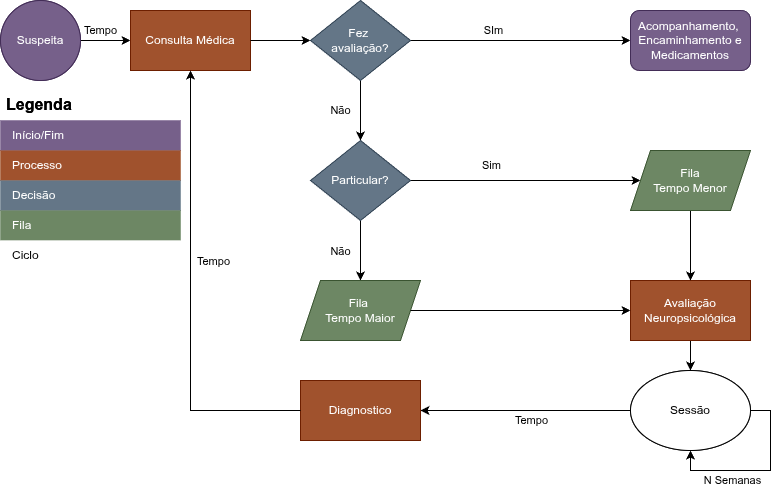
\includegraphics[width=10cm]{assets/fluxograma_pacientes_medicina.drawio.png}
	\label{fig:esboco_processo}
	\legend{Fonte: Elaborado pelos autores}
\end{figure}

Será adotada uma metodologia de desenvolvimento baseada em prototipação e simulação. Será inicialmente criado um modelo simplificado do processo contendo as principais etapas identificadas. Posteriormente, o modelo será refinado de acordo com os dados levantados e os gargalos encontrados. Com base nisso, serão executadas simulações com fim de comparar o funcionamento do processo em condições diferentes. Essa metodologia incremental permitirá o ajuste do modelo progressivamente, garantindo sua representação de forma mais adequada ao problema.

Os critérios de avaliação estão ligados com a capacidade do modelo de representação do processo de diagnóstico e da indicação de melhorias viáveis. Serão utilizadas métricas como tempo médio total até a devolução do diagnóstico, tempo médio de espera em cada etapa, tamanho das filas, taxa de utilização dos profissionais e identificação do principal gargalo do sistema. Ademais, simulações de cenários simulados serão comparadas entre si com o intuito de verificar as estratégias que apresentam melhores resultados no que diz respeito à redução do tempo de espera, mantendo a qualidade necessária para realizar uma avaliação confiável.


\section{Procedimentos da abordagem proposta}
Detalhe etapas da metodologia em ordem cronológica. Use listas numeradas, diagramas de fluxo ou pseudocódigo para tornar o processo claro.

\section{Ferramentas, tecnologias e ambientes}

% Liste softwares, linguagens, bibliotecas, frameworks e ambientes (laboratórios, nuvem, simulação) que serão usados. Justifique a escolha com base no problema e nas métricas.

Para o desenvolvimento do trabalho, utilizamos as seguintes ferramentas separadas por categoria:
\begin{itemize}
		\item \textbf{Linguagem de programação:} Python 3.13 ou superior, devido à sua ampla gama de bibliotecas voltadas para análise estatística, manipulação de dados e simulação de processos.
		\item \textbf{Bibliotecas:} Foram utilizadas tanto bibliotecas para a implementação da simulação e transformação de dados, quanto para validações de formatação de código, testes automatizados e padronização de mensagens de \textit{commit} no controle de versão, como:
		\begin{itemize}
			\item \textbf{Pandas:} utilizado para manipulação, análise e importação de dados, permitindo a organização e tratamento eficiente das informações coletadas. Com o Pandas, foi possível extrair diversos parâmetros para a simulação com base em uma planilha fornecida;
			\item \textbf{SimPy:} para simulação de eventos discretos, possibilitando a representação de filas, recursos e eventos ao longo do tempo. Com isso, é possível extrair métricas relevantes para a alteração de cenários;
			\item \textbf{Taskipy:} utilizado para definir comandos frequentemente usados, como a execução do simulador, dos testes automatizados, e da verificação da formatação do código;
			\item \textbf{Pytest:} Ferramenta de desenvolvimento de testes automatizados. Foram desenvolvidos tanto testes unitários, que validam as funções do código, quanto testes de confiabilidade, que validam os resultados da simulação em relação ao cenário real. Foi utilizado para garantir que as simulações tragam resultados corretos, e que as funções em todo o código estejam retornando resultados esperados e previsíveis;
			\item \textbf{Black:} Formatador e validador de formatação do código, que auxilia na leitura do código-fonte do projeto, mantendo uma padronização;
			\item \textbf{Commitizen}: Formatador e validador das mensagens de \textit{commit}, utilizado para manter um padrão das mensagens.
		\end{itemize}
		\item \textbf{Controle de versão:} Para o controle de versão, foi utilizado o git, que permite manter um histórico baseado em \textit{commits} (Registro de uma alteração realizada no projeto), além de possuir recursos que permitem a sincronização entre ambientes locais e remotos;
		\item \textbf{Automações de validação:} Foi utilizado o \textit{Github Actions} para validar os registros de alteração realizados no projeto, com o objetivo de validar toda alteração proposta através de \textit{Pull Requests}. A automação valida: Resultado dos testes automatizados, checagem de formatação de código com o \textit{black}, e checagem das mensagens de \textit{commit} com o \textit{commitizen};
		\item \textbf{Gerenciador de dependências:} Para gerenciar a declaração e as versões das dependências, foi utilizado o Poetry, permitindo que as dependências do projeto seja instalado a partir do comando \texttt{poetry install}.
\end{itemize}

Não foi utilizado nenhuma biblioteca que dependa de rede ou computação em nuvem, com isso, o trabalho pode ser executado em qualquer computador com Python instalado na versão 3.13 ou superior, juntamente com as dependências do projeto. Assim, a execução do simulador não tem a necessidade de conexão com a internet.

Com isso, o principal insumo externo do trabalho trata-se dos parâmetros fornecidos, que consiste em:
\begin{itemize}
	\item \textbf{Planilha de dados:} Lista de agendamentos dos exames de pacientes, contendo as seguintes colunas:
	\begin{itemize}
		\item \textbf{ID do Paciente:} identificador único do paciente;
		\item \textbf{ID do Profissional:} identificador único do profissional;
		\item \textbf{Início da agenda:} data e horário de início do exame, em formato \textit{ISO 8601} com fuso horário;
		\item \textbf{Fim da agenda:} data e horário do fim do exame, em formato \textit{ISO 8601} com fuso horário;
		\item \textbf{Suspeita do paciente:} qual diagnóstico o paciente busca, como autismo, TDAH, entre outros;
		\item \textbf{Status da agenda:} como está a situação da agenda. Os possíveis valores são: Pendente (Ainda não aconteceu a agenda), Falta (O paciente não compareceu), Concluída (O paciente compareceu na agenda);
		\item \textbf{ID de Agendamento (Opcional):} identificador da agenda apresentada
		\item \textbf{Nome do paciente (Opcional):} nome do paciente que participará da agenda. É utilizado apenas como nome de exibição, mas não é relevante para a simulação
		\item \textbf{Nome do profissional (Opcional):} nome do profissional que atenderá o paciente. É utilizado apenas como nome de exibição, mas não é relevante para a simulação;
	\end{itemize}	
	\item \textbf{Recursos e restrições:} parâmetros que podem ser inseridos para o simulador considerar, no lugar do que foi inserido na planilha, como:
	\begin{itemize}
		\item \textbf{Quantidade de profissionais:} o usuário pode simular com N profissionais, ao invés da quantidade apresentada na planilha.
		\item \textbf{Mínimo de exames por suspeita:} pode ser inserido nas parametrizações a quantidade mínima de exames para se obter um diagnóstico para determinada suspeita, e uma quantidade mínima padrão, que independe da suspeita.
	\end{itemize}
\end{itemize}

\section{Procedimentos experimentais e métricas}
Explique como os experimentos serão configurados, quais variáveis serão controladas e quais métricas demonstram que a proposta cumpre os objetivos (ex.: acurácia, latência, custo). Inclua tabelas que antecipem o plano de coleta, por exemplo:
\begin{table}[htb]
  \centering
  \caption{Plano de experimentação}
  \begin{tabular}{lccc}
    \toprule
    Experimento & Variável controlada & Métrica principal \\
    \midrule
    Comparação com baseline & algoritmo & acurácia \\
    Escalabilidade & carga & tempo médio \\
    \bottomrule
  \end{tabular}
  \legend{Exemplo de como documentar experimentos.}
\end{table}

\textit{Propor algo não basta: demonstre como será validado.}

% ---------------------------------------------------------------
% DESENVOLVIMENTO
% ---------------------------------------------------------------
\chapter{Desenvolvimento / Implementação / Experimentos}

\section{Modelagem e arquitetura}
Apresente diagramas (UML, blocos ou fluxogramas) que mostram como os módulos se relacionam, identificando componentes críticos e como eles atendem ao problema e à metodologia.

\section{Detalhes de implementação}
Explique escolhas tecnológicas, estruturas de dados e integrações. Inclua trechos de código relevantes ou pseudoexemplos se esclarecerem decisões de pesquisa.

\section{Experimentos e cenários de teste}
Descreva os cenários planejados, parâmetros testados e por que cada experimento está alinhado aos objetivos. Liste os conjuntos de dados, variações e número de repetições.

\section{Coleta e tratamento de dados}
Explique como os dados foram coletados (logs, sensores, APIs), armazenados e preparados (limpeza, normalização, anonimização). Registre ferramentas usadas no pré-processamento.

\textit{O desenvolvimento só é pesquisa se estiver claramente ligado ao problema e à metodologia definida.}

% ---------------------------------------------------------------
% RESULTADOS
% ---------------------------------------------------------------
\chapter{Resultados e Análise}

\section{Apresentação dos resultados}
Mostre resultados com tabelas, gráficos e figuras. Diferencie:
\begin{itemize}
  \item \textbf{Figura:} imagens, diagramas conceituais ou arquiteturais que ilustram estrutura ou fluxo.
  \item \textbf{Gráfico:} plot de dados (linhas, barras, boxplots) que compara métricas obtidas.
\end{itemize}

Exemplo de tabela:
\begin{table}[htb]
  \centering
  \caption{Comparação de métricas reportadas}
  \begin{tabular}{lcc}
    \toprule
    Método & Acurácia & Tempo médio (ms) \\
    \midrule
    Proposta & 92\% & 180 \\
    Baseline & 88\% & 220 \\
    \bottomrule
  \end{tabular}
  \legend{Tabela exemplificando como comparar métricas.}
\end{table}

Ao inserir um gráfico (por exemplo `assets/figures/desempenho.png`), use:
\begin{verbatim}
\begin{figure}[htb]
  \centering
  \includegraphics[width=0.8\textwidth]{assets/figures/desempenho.png}
  \caption{Gráfico de comparação das métricas de acurácia.}
  \label{fig:grafico-desempenho}
\end{figure}
\end{verbatim}

\section{Análise crítica e comparação}
Discuta as descobertas com base na revisão bibliográfica e na hipótese. Evidencie ganhos e perdas.

\section{Discussão}
Relacione os resultados aos objetivos e à hipótese, explicitando se o critério de sucesso foi atingido.

\textit{Resultados devem ser analisados, não apenas exibidos.}

% ---------------------------------------------------------------
% CONCLUSÃO
% ---------------------------------------------------------------
\chapter{Conclusão}

\section{Retomada do problema e dos objetivos}
Retome o problema e destaque o que foi atingido.

\section{Contribuições para a Computação}
Explique o que a pesquisa trouxe de novo.

\section{Limitações e trabalhos futuros}
Liste limites e sugira próximos passos coerentes.

% ---------------------------------------------------------------
% OBSERVAÇÕES DO AUTOR
% ---------------------------------------------------------------
\chapter*{Observações importantes}
\addcontentsline{toc}{chapter}{Observações importantes}

Para graduação, Wazlawick aceita trabalhos aplicados desde que:
\begin{itemize}
    \item O problema seja preciso;
    \item A solução esteja fundamentada;
    \item Haja análise crítica;
    \item Não seja apenas entrega funcional.
\end{itemize}

\postextual

\bibliography{bibliografia}

\end{document}
